\chapter{Background}
\label{ch:background}

In this chapter, we describe the theoretical framework in which this thesis operates. We will first introduce the observed phenomenon of mutations and the erroneous mutation matrix we receive from single-cell sequencing. Then, we will introduce the likelihood function we wish to maximize, and the mutation trees and attachment functions that we use to model the true mutation status of the cells. Lastly, we introduce the \ac{SCITE} Markov chain which uses all of the previous concepts to find a maximum-likelihood mutation tree. All of this is conceptually equivalent to the framework used by Jahn et al. \cite{tree2016}, but with enhanced precision and details. Equivalent formalizations are found in either the original paper or implementation if not indicated otherwise. First, we will formalize the observed phenomenon of mutations:

\begin{definition}[Mutation matrix]
    \label{def:mutmatrix}
    Let $C$ be the set of cells with $|C| \in \mathbb{N}$ and $G$ be the set of genes with $|G| \in \mathbb{N}$. Then, we define the random variables $E$ and $D$ with $\mathrm{im}(E) \subseteq \{0,1\}^{|C| \times |G|}$ and $\mathrm{im}(D) \subseteq \{0, 1, 2\}^{|C| \times |G|}$. $E$ is the true mutation matrix that describes the actual state of the cells, and $D$ is the observed, erroneous mutation matrix. Let also $\alpha \in (0,1)$ be the probability of false positives and $\beta \in (0,1)$ be the probability of false negatives. We then assume the following for all $c \in C, g \in G$:
    \begin{align*}
        \mathbb{P}(D_{c,g} = 1 \mid E_{c,g} = 0 \wedge D_{c,g} \neq 2) &:= \alpha & \mathbb{P}(D_{0,j} = 0\mid E_{c,g} = 1 \wedge D_{c,g} \neq 2) &:= \beta \\
        \mathbb{P}(D_{c,g} = 0 \mid E_{c,g} = 0 \wedge D_{c,g} \neq 2) &:= (1-\alpha) & \mathbb{P}(D_{c,g} = 1 \mid E_{c,g} = 1 \wedge D_{c,g} \neq 2) &:= (1-\beta)
    \end{align*}
    The additional prior $D_{c,g} \neq 2$ is not present in the original formalization, but technically necessary since we would otherwise have $\mathbb{P}(D_{c,g} = 2 \mid E_{c,g} = e) = 0$ for all $e \in \{0,1\}$, which is not useful.
    
    Although this thesis was initially very applied in nature, it has become very theoretical. Therefore, we have decided to use theoretical indexing conventions in this thesis. Therefore, we use the first index to indicate the column of the matrix and the second index to indicate the row. We also use 1 as our first index and upper index bounds are inclusive.
\end{definition}

\begin{definition}[Likelihood function]
    \label{def:likelihood}
    We define the elementary likelihood function $\lambda$ as follows:
    \begin{align*}
        \lambda_d: \{0, 1, 2\} \times \{0, 1\} \rightarrow [0, 1], (d, e) &\mapsto \begin{cases}
            1-\alpha & d = 0 \wedge e = 0 \\
            \alpha & d = 1 \wedge e = 0 \\
            \beta & d = 0 \wedge e = 1 \\
            1-\beta & d = 1 \wedge e = 1 \\
            1 & d = 2
        \end{cases}
    \end{align*}
    We, therefore, have 
    \begin{align*}
        \lambda(d_{c,g}, e_{c,g}) = \mathbb{P}(D_{c,g} = d_{c,g} \mid E_{c,g} = e_{c,g} \wedge D_{c,g} \neq 2)
    \end{align*}
    for all $d \in \{0,1,2\}^{n \times m}, e \in \{0,1\}^{n \times m}, g \in G, c \in C$ with $d_{c,g} \neq 2$. We make the distinction between $d_{c,g} = 2$ and $d_{c,g} \neq 2$ since we are not interested in lost data, with the underlying assumption that data loss is independent of the true mutation status of a cell. This distinction is not present in the original formalization, but it is present in the original implementation. Given an observed mutation data matrix $d \in \{0,1,2\}^{n \times m}$, we then define the global likelihood function as follows:
    \begin{align*}
        \Lambda_d : \{0,1\}^{|C| \times |G|} \rightarrow [0,1], e \mapsto \prod_{c \in C} \prod_{g \in C} \lambda(d_{c,g}, e_{c,g})
    \end{align*}
\end{definition}

This function $\Lambda_d$ is the likelihood function we wish to maximize. We could now define the problem using only mutation matrices, but since Jahn et al. make no statement whether \ac{SCITE} also finds the maximum-likelihood mutation matrix, we restrict ourselves to maximum-likelihood mutation trees, which we will define now:

\begin{definition}[Mutation trees]
    \label{def:mutation_tree}
    Let $G$ be the set of considered genes. A mutation tree is a rooted, directed tree $T = (V, E, r)$ with $V = G \cup \{r\}$. We, therefore, have $E \subseteq V^2$ and $|V| = |G| + 1$.
\end{definition}

\begin{definition}[Tree-related notations]
    \label{def:reachability}
    Let $T = (V, E)$ be a tree and $v, w \in V$. $w$ is reachable from $v$, formally $v \leadsto_T w$, iff there is a path $p = (v, \dots, w)$ in $T$. We also define the parent of $v$, formally $p_T(v) \in V$, as the node with $(p_T(v), v) \in E$ if such a node exists. These notations are generally well known and do not necessarily need an introduction, but we want to assure that the reader is aware of them.
\end{definition}

\begin{definition}[Attachment functions]
    \label{def:attachment}
    Let $C$ and $G$ be the set of considered cells and genes, respectively, and $T$ a mutation tree. An attachment function is a function $\sigma: C \rightarrow V$ that maps cells onto tree nodes.
\end{definition}

\begin{definition}[Induced mutation matrix]
    \label{def:induced_mutmatrix}
    Let $C$ and $G$ be the set of considered cells and genes, respectively, $T$ be a mutation tree and $\sigma$ be an attachment function. We define the mutation matrix $e_{T, \sigma} \in \{0,1\}^{|C| \times |G|}$ induced by the mutation matrix and attachment function as follows:
    \begin{align*}
        \forall c \leq C, g \leq G: (e_{T, \sigma})_{c,g} := \begin{cases}
            1 & g \leadsto_T \sigma(c) \\
            0 & \mathrm{else}
        \end{cases}
    \end{align*}
    This means that a cell $c$ has a mutation at the gene $g$ iff $g$ is an ancestor of its attachment node $\sigma(c)$. An example of an induced mutation matrix is found in example \ref{exmpl:scite_problem}.
\end{definition}

\begin{definition}[The SCITE problem]
    \label{def:scite_problem}
    Let $C$ and $G$ be the set of considered cells and genes, respectively, and $d \in \{0,1\}^{|C| \times |G|}$ an observed mutation matrix. The \ac{SCITE} problem is: Find a mutation tree $T$ and an attachment function $\sigma$ so that $\Lambda_d(e_{T, \sigma})$ is maximal.
\end{definition}

\begin{example}
    \label{exmpl:scite_problem}
    We consider 4 cells and 4 genes in this example and therefore set $C = \{1,2,3,4\}$ and $G = \{1,2,3,4\}$. We assume that the true, underlying mutation tree $T$ and attachments $\sigma$ look like this:
    \begin{center}
        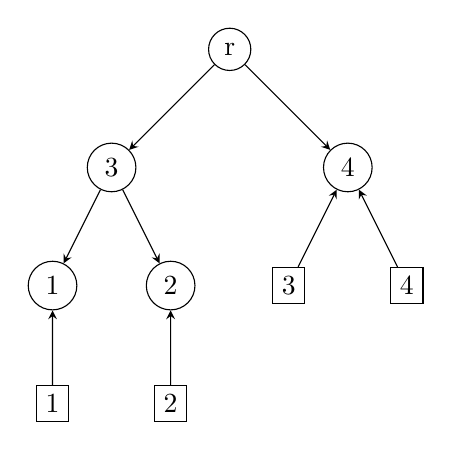
\begin{tikzpicture}
            \draw[every node/.style={draw}, level 1/.style={sibling distance=3cm}, level 2/.style={sibling distance=1.5cm}, edge from parent/.append style={-stealth}]
                node[circle] {r}
                child {
                    node[circle] {3} 
                    child {
                        node[circle] {1}
                        child {node {1} edge from parent[stealth-]}
                    }
                    child {
                        node[circle] {2}
                        child {node {2} edge from parent[stealth-]}
                    }
                }
                child {
                    node[circle] {4}
                    child {node {3} edge from parent[stealth-]}
                    child {node {4} edge from parent[stealth-]}
                };
        \end{tikzpicture}
    \end{center}
    In this graph, the encircled nodes represent the actual nodes of the mutation tree, while the squared nodes represent cells that are attached to a node. Therefore, this gives us the following true, induced mutation matrix:
    \begin{align*}
        e_{T, \sigma} &= \begin{pmatrix}
            1 & 0 & 0 & 0 \\
            0 & 1 & 0 & 0 \\
            1 & 1 & 0 & 0 \\
            0 & 0 & 1 & 1 \\
        \end{pmatrix}
    \end{align*}
    For example, cell number 1 is attached to node number 1, which means that we have $\sigma(1) = 1$. Since only nodes 1 and 3 are on the path from the root to the attachment point $\sigma(1)$, there are 1-entries exactly at positions $(1,1)$ and $(3,1)$ of $e_{T, \sigma}$, but not at $(2,1)$ and $(4,1)$.
    
    We now assume that $(\alpha, \beta) = (0.01, 0.4)$ and that matrix entries are reported as missing with a probability of 0.25, after the false-positive and false-negative errors are decided. This is not necessarily the case for all inputs or the real world, but we can use this model to generate an observed mutation matrix $d$, like this one:
    \begin{align*}
        d &= \begin{pmatrix}
            1 & 0 & 0 & 0 \\
            0 & 2 & 0 & 2 \\
            1 & 1 & 2 & 0 \\
            0 & 0 & 0 & 1 \\
        \end{pmatrix}
    \end{align*}
    Now, we can compute the likelihood of the underlying mutation tree and attachment:
    \begin{align*}
        \Lambda_d(e_{T, \sigma}) = (1-\alpha)^{8} \cdot \alpha^{0} \cdot (1-\beta)^{4} \cdot \beta^{1} &\approx 0.05 \\
        &\approx \exp(-3.04)
    \end{align*}
    However, if you attach cell 3 to gene 3 instead, you get the following tree:
    \begin{center}
        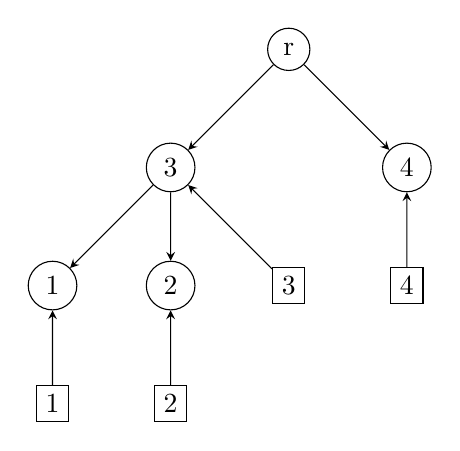
\begin{tikzpicture}
            \draw[every node/.style={draw}, level 1/.style={sibling distance=3cm}, level 2/.style={sibling distance=1.5cm}, edge from parent/.append style={-stealth}]
                node[circle] {r}
                child {
                    node[circle] {3} 
                    child {
                        node[circle] {1}
                        child {node {1} edge from parent[stealth-]}
                    }
                    child {
                        node[circle] {2}
                        child {node {2} edge from parent[stealth-]}
                    }
                    child {node {3} edge from parent[stealth-]}
                }
                child {
                    node[circle] {4}
                    child {node {4} edge from parent[stealth-]}
                };
        \end{tikzpicture}
    \end{center}
    with the following true mutation matrix:
    \begin{align*}
        e_{T, \sigma'} = \begin{pmatrix}
            1 & 0 & 0 & 0 \\
            0 & 1 & 0 & 0 \\
            1 & 1 & 1 & 0 \\
            0 & 0 & 0 & 1 \\
        \end{pmatrix}
    \end{align*}
    and the following likelihood:
    \begin{align*}
        \Lambda_d(e_{T, \sigma'}) = (1-\alpha)^{9} \cdot \alpha^{0} \cdot (1-\beta)^{4} \cdot \beta^{0} &\approx 0.12 \\
        &\approx \exp(-2.13) 
    \end{align*}
    This is one of the solutions found by \ac{SCITE}. This shows that the true, underlying mutation tree and attachment function is not necessarily the most likely one. It is not easy to tell whether this is a problem with the model itself or whether this information is simply lost in the errors. However, we have decided to not look into this issue as it does not align with our goals.
\end{example}

Next, we have a lemma that shows that it is not necessary to search for the maximal attachment function given a mutation tree:

\begin{lemma}[Maximum-likelihood attachment function]
    \label{lem:max_attachment}
    Let $C$ and $G$ be the set of considered cells and genes, respectively, $d \in \{0,1\}^{|C| \times |G|}$ an observed mutation matrix, and $T$ a mutation tree. We define:
    \begin{align*}
        \sigma_{\max, T}: C \rightarrow V, c \mapsto \argmax_{v \in V} \prod_{g \in G} \lambda \left(d_{c,g}, \begin{cases}
            1 & g \leadsto_T v \\
            0 & \mathrm{else} \\
        \end{cases}\right)
    \end{align*}
    $\sigma_{\max, T}$ maximizes $\Lambda_d (e_{T, \sigma})$ among all $\sigma: C \rightarrow V$.
\end{lemma}

Informally, $\sigma_{\max, T}$ simply picks the most-likely attachment node for every individual cell and using this attachment function yields the maximum likelihood for every tree, respectively. This lemma is already assumed to be true in the original SCITE paper \cite{tree2016}. Therefore, we see no need to prove it. However, it means that we only need to try different trees, not tree-attachment combinations, and we can simply write $\Lambda_d(T)$ instead of $\Lambda_d(e_{T, \sigma_{\max, T}})$ to express the likelihood of a mutation tree. Now, we can finally describe the \ac{SCITE} Markov chain and algorithm:

\begin{definition}[SCITE Markov chain, \cite{tree2016}]
    We define the \ac{SCITE} Markov chain as the Markov chain $(T_i)_{i \in \mathbb{N}_0} \in \{(V, E, r) : (V, E, r) \text{ is mutation tree}\}$. $T_0$ is uniformly distributed over the set of all mutation trees, and for every $i \in \mathbb{N}_0$, we set $T_{i+1} := \textsc{ChainStep}(T_i)$.
\end{definition}

The \textsc{ChainStep} algorithm (Algorithm \ref{alg:scite-step}) works by introducing one of three modifications to the tree and accepting it as the new state with a probability related to the increase in likelihood. The first of these modifications is the ``swap nodes'' move. In this move, two distinct non-root nodes $v$ and $w$ are sampled and their position in the tree is swapped. The resulting edge set is just defined as the original edge set where every occurrence of $v$ and $w$ are swapped. ``swap nodes'' is therefore also referred to as ``label swap'' since if the node-gene relationship were modeled with a node labeling function, one would simply need to swap the labels of $v$ and $w$. The next and most basic modification is ``prune and reattach.'' In this move, a node $v$ is sampled from all non-root nodes and a node $w$ is sampled from all nodes that are not descendants of $v$, including the root $r$. Then, the node $v$ is simply attached to $w$. Lastly, there is the ``swap subtrees'' modification. Here, two distinct non-root nodes $v$ and $w$ are sampled too. If $v$ and $w$ are unrelated (formally $v \not\leadsto_T w \wedge w \not\leadsto_T v$), $v$ is simply attached to $w$'s former parent and $w$ is attached to $v$'s former parent. However, if we have $w \leadsto_T v$, a third node $t$ is sampled from all descendants of $v$ and $w$ is attached to $t$ instead of $v$'s parent. This assures that no circles are introduced to the tree. If we have $v \leadsto_T w$, we can simply swap $v$ and $w$ and do the same.

If we would now accept every modified tree, we would eventually encounter a high- or even maximum-likelihood tree. However, the probability of this is low since the chain wanders through the search space aimlessly. Therefore, Jahn et al. employed a rejection sampling method that accepts solutions with a high likelihood and rejects solutions with a low likelihood. The exact way how this is achieved is documented in algorithm \ref{alg:scite-step} and according to the authors, this assures that the chain converges on trees with a high likelihood.
    
The \ac{SCITE} algorithm simulates the \ac{SCITE} Markov chain for a user-requested number of steps and repetitions and outputs the state $T$ with the highest $\Lambda_d(T)$ it has encountered. The goal of the thesis is to simulate the \ac{SCITE} Markov chain as quickly as possible, at least as quickly as the original implementation.

\begin{algorithm}[p]
    \begin{algorithmic}[1]
        \Function{ChainStep}{$T$}
            \State $(V, E, r) \leftarrow T$
            \State $\mathrm{move} \leftarrow \text{sample uniformly from } \{\text{``swap nodes''}, \text{``prune and reattach''}, \text{``swap subtrees''}\}$
            \If{$\mathrm{move} = \text{``swap nodes''}$}
                \State $v \leftarrow \text{sample uniformly from } V \setminus \{r\}$
                \State $w \leftarrow \text{sample uniformly from } V \setminus \{r, v\}$
                \State $f : V \rightarrow V, x \mapsto \begin{cases}
                    w & x = v \\
                    v & x = w \\
                    x & \text{else} \\
                \end{cases}$
                \State $E' \leftarrow \{(f(x), f(y)) : (x, y) \in E\}$
                \State $f_\mathrm{correction} \leftarrow 1$
            \ElsIf{$\mathrm{move} = \text{``prune and reattach''}$}
                \State $v \leftarrow \text{sample uniformly from } V \setminus \{r\}$
                \State $w \leftarrow \text{sample uniformly from } \{w \in V : v \not\leadsto_T w\}$
                \State $E' \leftarrow \left(E \setminus \{(p_T(v), v)\}\right)  \cup \{(w, v)\}$ \Comment Remove the old edge, add the new one
                \State $f_\mathrm{correction} \leftarrow 1$
            \ElsIf{$\mathrm{move} = \text{``swap subtrees''}$}
                \State $v \leftarrow \text{sample uniformly from } V \setminus \{r\}$
                \State $w \leftarrow \text{sample uniformly from } V \setminus \{r, v\}$
                \If{$v \leadsto_T w$}
                    \State $v, w \leftarrow w, v$ \Comment Ensure that $v$ is always a descendant or unrelated to $w$.
                \EndIf
                \If{$w \leadsto_T v$}
                    \State $t \leftarrow \text{sample uniformly from } \{x \in V: v \leadsto_T x\}$
                    \State $f_\mathrm{correction} \leftarrow \frac{|\{x \in V : v \leadsto_T x\}|}{|\{x \in V : w \leadsto_T x\}|}$
                \Else
                    \State $t \leftarrow p(v)$
                    \State $f_\mathrm{correction} \leftarrow 1$
                \EndIf
                \State $E' \leftarrow (E \setminus \{(p_T(v), v)\}) \cup \{(p_T(w), v)\}$ \Comment Remove the old edge to $v$, add the new one
                \State $E' \leftarrow (E' \setminus \{(p_T(w), w)\}) \cup \{(t, w)\}$ \Comment The same as above for $w$
            \EndIf
            \State $T' \leftarrow (V, E', r)$
            \If{accept with probability $\left(f_\mathrm{correction} \cdot \frac{\Lambda_d(T')}{\Lambda_d(T)}\right)$}
                \State \Return $T'$
            \Else
                \State \Return $T$
            \EndIf
        \EndFunction
    \end{algorithmic}
    \caption{Algorithm to compute the next chain step of a SCITE Markov Chain, adapted from \cite{tree2016}}
    \label{alg:scite-step}
\end{algorithm}

\begin{example}
    \label{exmpl:chain_step}
    We will give examples of different chain steps. We use the same tree as in example \ref{exmpl:scite_problem}, but without the attached cells since these are not relevant now:
    \begin{center}
        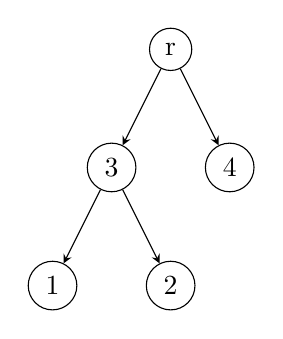
\begin{tikzpicture}
            \draw[every node/.style={draw}, edge from parent/.append style={-stealth}]
                node[circle] {r}
                child {
                    node[circle] {3} 
                    child { node[circle] {1} }
                    child { node[circle] {2} }
                }
                child { node[circle] {4} };
        \end{tikzpicture}
    \end{center}
    If we now execute a ``swap nodes'' move with $v = 3$ and $w = 4$, the resulting tree looks like this:
    \begin{center}
        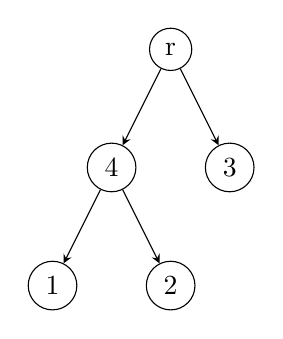
\begin{tikzpicture}
            \draw[every node/.style={draw}, edge from parent/.append style={-stealth}]
                node[circle] {r}
                child {
                    node[circle] {4} 
                    child { node[circle] {1} }
                    child { node[circle] {2} }
                }
                child { node[circle] {3} };
        \end{tikzpicture}
    \end{center}
    Nodes 4 and 3 just have swapped their labels. Everything else is still the same. Now, we execute the ``prune and reattach'' move with $v = 4$ and $w = 3$, so we take node 4 and attach it to node 3. This is possible since there is no path from node 4 to node 3:
    \begin{center}
        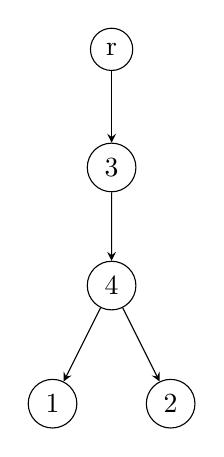
\begin{tikzpicture}
            \draw[every node/.style={draw}, edge from parent/.append style={-stealth}]
                node[circle] {r}
                child {
                    node[circle] {3}
                    child {
                        node[circle] {4} 
                        child { node[circle] {1} }
                        child { node[circle] {2} }
                    }
                };
        \end{tikzpicture}
    \end{center}
    Now, we will give an example of the ``swap nodes'' move with related subtrees. Firstly, we choose $v = 4$ and $w = 3$. Since we have $w \leadsto_T v$, we don't need to swap $v$ and $w$, but we need to sample a new target node $t$ among the descendants of $v$. Since every node is also its own descendant, we can choose $t = v = 4$. Now, we attach $v = 4$ to $r$, which is the parent of $w = 3$, and attach 3 to $t = 4$. The resulting tree looks like this:
    \begin{center}
        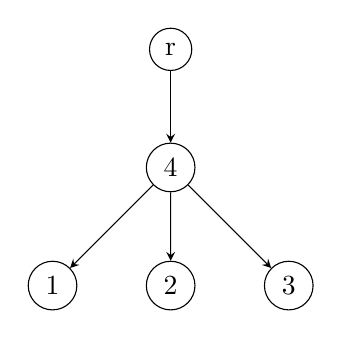
\begin{tikzpicture}
            \draw[every node/.style={draw}, edge from parent/.append style={-stealth}]
                node[circle] {r}
                child {
                    node[circle] {4} 
                    child { node[circle] {1} }
                    child { node[circle] {2} }
                    child { node[circle] {3} }
                };
        \end{tikzpicture}
    \end{center}
\end{example}